\documentclass{article}
\usepackage[utf8]{inputenc}

\title{DiSH - Detecting Subspace cluster Hierarchies \\ Data Mining- Assignment 1}
\author{Konrad Johannes Rüdiger von Kirchbach, Donatella Novakovic, \\ Wolfgang Martin Ost, Jakob Weber}
\date{November 2018}

\usepackage{natbib}
\usepackage{graphicx}
%\usepackage{algorithm}
\usepackage{algorithmic}
\usepackage{algpseudocode}
\algnewcommand\algorithmicforeach{\textbf{for each}}
\algdef{S}[FOR]{ForEach}[1]{\algorithmicforeach\ #1\ \algorithmicdo}
\usepackage{subfigure}


\begin{document}

\maketitle

\section{Introduction}
DiSH (Detecting Subspace cluster Hierarchies) belongs to the group of subspace clustering algorithms and is an advanced version of HiSC (Finding Hierarchies of Subspace Clusters) considering the discovery of more complex hierarchies. Both, DiSH and HiSC are subspace clustering methods based on OPTICS (Ordering points to identify the clustering structure). DiSH is intended to eliminate the limitations of clustering algorithms given by the approach of generating non-overlapping clusters. More precisely, these algorithms assign points uniquely to one cluster or noise. The aim of DiSH is to enable improvement in following properties over the state-of-the-art subspace clustering approaches\cite{achtert2007detection}: 
\begin{itemize}
    \item Uncovering of complex hierarchies of nested subspace clusters
    \item Detection of clusters in subspaces of different dimensionality
    \item Ability to detect clusters of different size, shape and density
\end{itemize}

This elaboration deals with the implementation of the algorithm DiSH according to explanations and findings of Achtert et al.\cite{achtert2007detection} and the further comparison of results with the algorithms implemented in Environment for DeveLoping KDD-Applications Supported by Index-Structures (ELKI). The clustering result is evaluated using ???? metrics provided by the python scikit-learn package\footnote{https://scikit-learn.org/stable/modules/clustering.html}. The DiSH algorithm is first evaluated on a genereated synthetic data set, which shall point out the properties and advantages of this method. Secondly, as the Achtert et al. suggest, the Wages\footnote{htpp://lib.stat.cmu.edu} data set is used. Results of both data sets are evaluated using the implemented DiSH algorithm and compared to the DiSH algorithm implemented in ELKI.    

\section{Implementation}
This section discusses the approach of implementing the algorithm DiSH and addresses occurring difficulties and uncertainties during this task. The implementation process is fully based on the paper \emph{Detection and Visualization of Subspace Cluster Hierarchies}, published by E. Alchert et al. , which describes the the structure and procedure of DiSH. Following pseudo codes are adapted from the paper:\par

\begin{algorithm}
\caption{DiSH (D, \mu, \epsilon)}
\begin{algorithmic}
\STATE $co \leftarrow$ cluster order; \COMMENT{initially empty}
\STATE $pq \leftarrow$ empty priority queue ordered by \mathcal $REACHDIST_{\mu};$
\ForEach{$p \in D$}
\STATE compute $w(p)$;
\STATE \mathcal $p.REACHDIST_{\mu} \leftarrow \infty$;
\STATE insert $p$ into $pq$;
\WHILE{$pq$ \neq $0$}
\STATE $o$ \leftarrow $pq.next()$; \\
\STATE $\mu$-nearest neighbor of o w.r.t. $SDIST$;
\ForEach{$p$ \in $pq$}
\STATE $new_sr$ \leftarrow $max(SDIST(o, r), SDIST(o, p))$;
\STATE $pq.update(p, new_sr)$;
\STATE append $o$ to $co$;
\RETURN{$co$};
\end{algorithmic}
\label{The algorithm DiSH}
\end{algorithm}

\begin{algorithm}
\caption{method extractCluster(ClusterOrder $co$)}
\begin{algorithmic}
\STATE $cl$ \leftarrow empty list; \COMMENT{cluster list}
\ForEach{$o$ \in $co$}
\STATE $p$ \leftarrow $o.predecessor$;
\IF{ \nexists $c$ \in $cl$ with $w(c) = w(o,p)$ \wedge \mathcal $dist_{w(o,p)}(o, c.center)$ \leq $2*$ \epsilon}
\STATE create a new $c$;
\STATE add $c$ to $cl$;
\STATE add $o$ to $c$;
\RETURN{$cl$};
\end{algorithmic}
\label{Method for ectracting clusters from the cluster order}
\end{algorithm}

\begin{algorithm}
\caption{method buildHierarchy($cl$)}
\begin{algorithmic}
\STATE $d$ \leftarrow dimensionality of objects in D;
\ForEach{\mathcal $c_{i}$ \in $cl$}
\ForEach{\mathcal $c_{j}$ \in $cl$}
\IF{\mathcal (\lambda_{cj} > \lambda_{ci})}
\STATE $d$ \leftarrow \mathcal $dist_{w(ci, cj)}(ci.center, cj.center)$;
\IF{(\mathcal \lambda_{cj} = $d$ \vee (\emph{$d$} \leqq 2 * \epsilon \wedge \nexists$c$ \in $cl$ : $c$ \in $ci.parents$ \wedge \mathcal \lambda_{c} < \mathcal\lambda_{cj}))}
\STATE add \mathcal $c_{i}$ as child to \mathcal $c_{j}$
\end{algorithmic}
\end{algorithm}

The main idea of DiSH is the definition of the subspace distance. So, small values are assigned if two points are in a common low-dimensional subspace cluster, whereas high values are an indicator of two points in a common high-dimensional subspace cluster or in no subspace cluster at all. Consequently, subspace clusters with a small subspace distance are embedded within clusters with a higher subspace distances.\par

The subspace dimensionality for each point $o$ in the data set $D$ is computed, assuming that the optimal subspace has the highest dimensionality or a higher number of points in the neighborhood. This step is accomplished by analyzing the variance and considering only dimensions of low variance.  In other words, attributes $a$ become a candidate for a subspace if an attribute-wise $\epsilon$ query yields at least $\mu$ objects. Subsequently, these attributes must be combined in an optimal way. Therefore, we used the heuristic best-first search approach, presented in the paper, which scales linearly in the number of dimensions. Using this approach we can determine the subspace preference vectors $w(o)$. Only attributes with predicate 1 remain relevant, since these lead to the clusters. In the next step a similarity measure is defined, assigning the corresponding distance. In order to distinguish between points which are associated to the same k-dimensional subspace cluster and points associated to different k-dimensional subspace clusters, but intersect, it must be checked whether preference vector of two points are equal or if one preference vector is included in the other one. If the distance between the points in the subspace spanned by w(p,q) exceeds $2*\epsilon$, we can assume that the point belongs to parallel or intersected clusters. Similar to OPTICS, also here the distance within a subspace cluster is considered, such that the subspace clusters can exhibit arbitrary sizes shapes and densities. A factor $\mu$ is introduced and represents the minimum number of points in a cluster to achieve robustness against noise points. A so-called cluster order is extracted which constructs an order of all points using the subspace reachability distance, where $r$ is supposed to be the $\mu$-nearest neighbor w.r.t the subspace distance of $p$. Due to the data structure, for this step a naive approach running trough every single data point was our best alternative.\par  

%Heuristic Approach Pseudo Code?

However, several ambiguities arose during the implementation of DiSH. Due to some missing details and explanations in the paper, the task of implementing DiSH became rather complex. Variables, such as \emph{predecessor}, used in method \emph{extractCluster} lack of explanation in the text. Also terms, such as $\mu - nearest neighbor of o w.r.t. SDIST$ are missing some clarification, since it can be understood differently. Either $\mu -nearest neighbor$ in the computed subspace or $\mu -nearest neighbor$ across all given dimensions. Furthermore, we also noticed some inconsistencies and confusions given the naming of variables used in the pseudo code. Looking at the method \emph{buildHierachy}, variable $d$ is used obviously in two different contexts, which can lead to confusion and extend the time of work.    
\section{Evaluation and Comparison of Results with ELKI}

In order to evaluate the implemented DiSH algorithm, we generated a synthetic data set which intends to illustrate the algorithms properties. Since the paper states that none of the existing algorithms succeeded in detecting hierarchical relationships among the subspace clusters, we created the data set in such a way that one 1D cluster is embedded within two 2D clusters and tested the performance in clustering. The parameters were determined as follows: $\epsilon = 0.01$, $\mu = 50$. The same parameters were used in both implementations: executing the implemented DiSH algorithm and executing the algorithm DiSH implemented in ELKI. Figure XY shows a suitable result. There exist two 2D clusters colored in purple and green. The 1D clusters is detected in the intersection colored in blue. 


\begin{figure}[h!]
\centering
    \subfigure[Clustering result using implemented DiSH on synthetic data set]{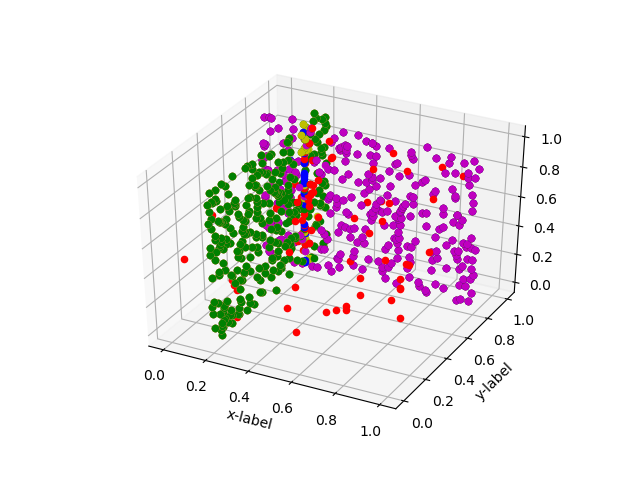
\includegraphics[width = 0.49\textwidth]{impl_synth_blau.png}}
    \subfigure[Clustering result using ELKI DiSH on synthetic data set]{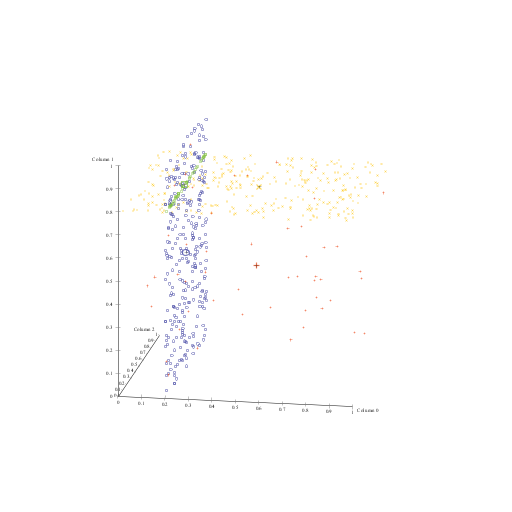
\includegraphics[width=0.49\textwidth]{elki_synth.png}}
\end{figure}


We also applied the implemented DiSH algorithm to the Wages data set, using the same parameter and information stated in the paper. Thus, we used the parameter values $\epsilon = 0.001$ and $\mu = 9$. Also we used only the stated dimensions:\emph{years of education},\emph{wage}, \emph{age} and \emph{years of work experience}, for clustering. 

\begin{figure}[h!]
\centering
    \subfigure[Clustering result using ELKI DiSH on data set: Wages]{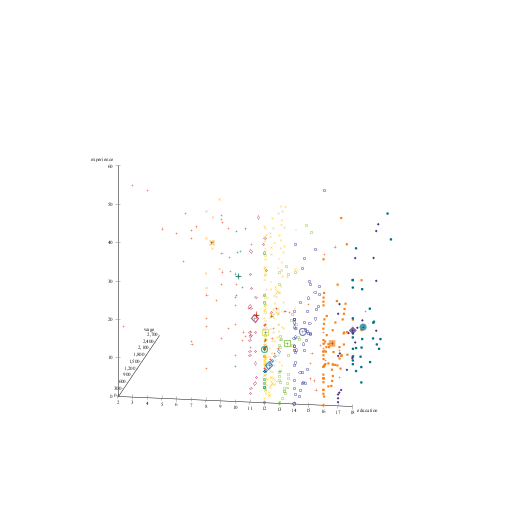
\includegraphics[width = 0.55\textwidth]{elki_wage.png}}
    \subfigure[Cluster Hierarchy; data set: Wages]{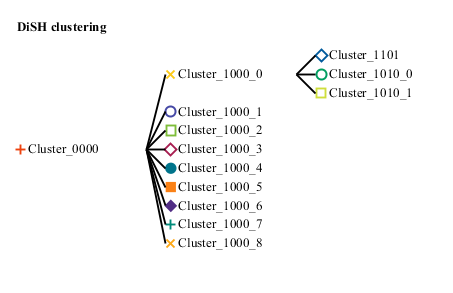
\includegraphics[width=0.40\textwidth]{elki_cluster_hierarchy.PNG}}
\end{figure}

\end{document}


